\documentclass[journal]{IEEEtran}

\hyphenation{op-tical net-works semi-conduc-tor}

\usepackage{cite}
\usepackage{amsmath,amssymb,amsfonts}
\usepackage{algorithmic}
\usepackage{graphicx}
\usepackage{textcomp}
\usepackage{xcolor}
\usepackage[linesnumbered,ruled,vlined]{algorithm2e}
\usepackage{hyperref}
\usepackage{graphicx}
\usepackage{float}
\usepackage{caption}

\begin{document}

\title{RAID-6 Based Distributed Storage System}

\author{Meng Shen,
        Ruihang Wang,
        Yihang Li % <-this % stops a space
\thanks{Meng shen and Ruihang Wang are with the School
of Computer Science Engineering, Nanyang Technological University, Singapore,
e-mail: (meng005@e.ntu.edu.sg, ruihang001@e.ntu.edu.sg).}% <-this % stops a space
\thanks{Yihang Li is with the School
of Electrical and Electronic Engineering, Nanyang Technological University, Singapore,
e-mail: (leah9704@gmail.com).}% <-this % stops a space
\thanks{Project submitted on Nov 23, 2019.}}

% The paper headers
\markboth{CE7490 2019 Fall - Advanced Topics in Distributed System - Project 2}%
{Shell \MakeLowercase{\textit{et al.}}: Bare Demo of IEEEtran.cls for IEEE Journals}

% make the title area
\maketitle

\begin{abstract}
RAID-6 is an extension of RAID-5 by adding another parity block. It is designed to tolerate any two concurrent disk failure and maintain a relatively high storage efficiency. The mathematics behind RAID-6 is Galois Field theory and Reed-Solomon Coding. In this project, we create our own finite field operation library and use it to develop a RAID-6 based distributed storage system in Python 3.7 under Linux envrionment. In addition to basic functionalities, we also developed several advanced features in the system that can accommodate real files of arbitrary size and support user defined configurations. To make it available for implementation, we open-source our codes with read-me documents at \url{https://github.com/GuluDeemo/CE7490-RAID6}
\end{abstract}

% Note that keywords are not normally used for peerreview papers.
\begin{IEEEkeywords}
RAID-6, Galois Field, Reed-Solomon codes, Python. 
\end{IEEEkeywords}


\section{Introduction}
\IEEEPARstart{T}{he} concept of RAID (Redundant Array of Independent Disks) was raised in  paper "A Case for Redundant Arrays of Inexpensive Disks (RAID)"\cite{IEEEhowto:kopka} for the demand of rising the reliability, capacity and speed of storage systems cost-efficiently. Instead of reading and writing data in one large disk drive, RAID organizes a series of inexpensive independent disk drives with certain patterns and offer a virtually unified disk drive. The idea of RAID achieved great performance with large capacity, wide width of input/output and low cost and hence gained popularity. Since 1970s, many versions of RAID have been raised according to requirements of different application scenarios and are widely used in various data protection applications. Most RAID versions implement error-detection drives and employ error-protection schemes called "parity" to provide fault tolerance ability in one or more disks. The most typical method is to generate a parity disk by simple XOR function, where failure of up to one disk can be tolerated by reconstructing the failed one from the rest of disk array. Other methods are designed for multiple failure tolerance, including Galois Field and Reed-Solomon error detection, which is used in RAID-6. This report will give an introduction of RAID family and then focus on the methodology and implementation of RAID-6.

Among all levels of RAID, RAID-5 and RAID-10 are most widely used by industry manufacturers. RAID-10 combines RAID-1 and RAID-0 by dividing data into several parts and mirroring each part into pairs. RAID-10 is designed to tolerate multiple disk failure except two corresponding disks in the mirroring pairs. However, the storage efficiency is only 50\% and can tolerant, which is very low. RAID-5 consists of block-level striping with distributed parity, and the parity information is saved among drives. When facing failure, the loss data can be calculated and rebuilt by distributed parity. However, RAID-5 can only tolerate one disk failure. RAID-6 is designed to tolerate any two concurrent disk failure and maintain a relatively high storage efficiency.

RAID-6 is a private raid-level standard proposed concurrently by several large enterprises. This RAID level is developed on the basis of RAID-5, while unlike RAID-5, there is not only a parity area for sibling data on the drive, but also a parity area for each data block. Two independent parity systems use different algorithms and the data is very reliable. Even if two disks fail at the same time, it does not affect the use of the data, which enhances the disk’s fault tolerance. With a RAID-6 based distributed storage system, it is possible to mitigate most of the problems associated with RAID-5.

RAID-6 achieves faster reading performance and higher fault tolerance. All these advantages make larger RAID groups more practical, especially for high-availability systems, as larger-capacity drives take longer to restore. The larger the drive capacities and the larger the array size, the more important it becomes to choose RAID-6 instead of RAID-5. However, RAID-6 is not as popular as other levels of RAID for practical application because of its complicated system and expensive RAID controller. For most small businesses which do not require high security level of data preservation, it is better to use RAID-5 economically. While for businesses demand higher security level of data preservation like data center, it is necessary to implement RAID-6.

In this report, we present a reliable distributed storage system based on RAID-6 under Python 3.7 environment. The mathematical operation in Galois Field is well investigated and created as a library to support RAID-6 controller through practical implementation. The RAID-6 based system support several basic functionalities, such as distributed data storage, failure detection and lost redundancy recovery. On top of the minimal implementation, we also developed several advanced features that can accommodate real files of arbitrary size and support various user-defined configurations for practical applications. The rest of the report is organized as follows: Section \ref{sec2} presents the overview of our project. Section \ref{sec3} investigates the mathematics and principle of RAID-6 system. Section \ref{sec4} introduces the implementation details of our designed system. Section \ref{sec5} presents experiment results of different configurations. The implementation of this project is concluded in Section \ref{sec6}.

\section{Overview}
\label{sec2}
The RAID-6 distributed storage system is developed in Python 3.7 under Linux environment. Instead of using existing finite field libraries, we create our own Galois Field \textbf{GF($2^8$)} operations based on the tutorial document of Reed-Solomon Coding in \cite{RAID-6}, \cite{tutorial}. The only dependency we use in this project is \emph{NumPy} for basic matrix operations. The functionalities we have developed for this RAID-6 system are summarized as follows:
\begin{itemize}
	\item Store and access abstract “data objects” across storage nodes using RAID-6 for fault-tolerance.
	\item Include mechanisms to determine failure of storage nodes.
	\item Carry out rebuild of lost redundancy at a replacement storage node.
	\item Accommodate real files of arbitrary size, taking into account issues like RAID mapping, etc. 
	\item Support mutable files, taking into account update of the content, and consistency issues.
	\item Support larger set of configurations
\end{itemize}

\begin{figure}[htbp]

	\centering

	\captionsetup{justification=centering}

	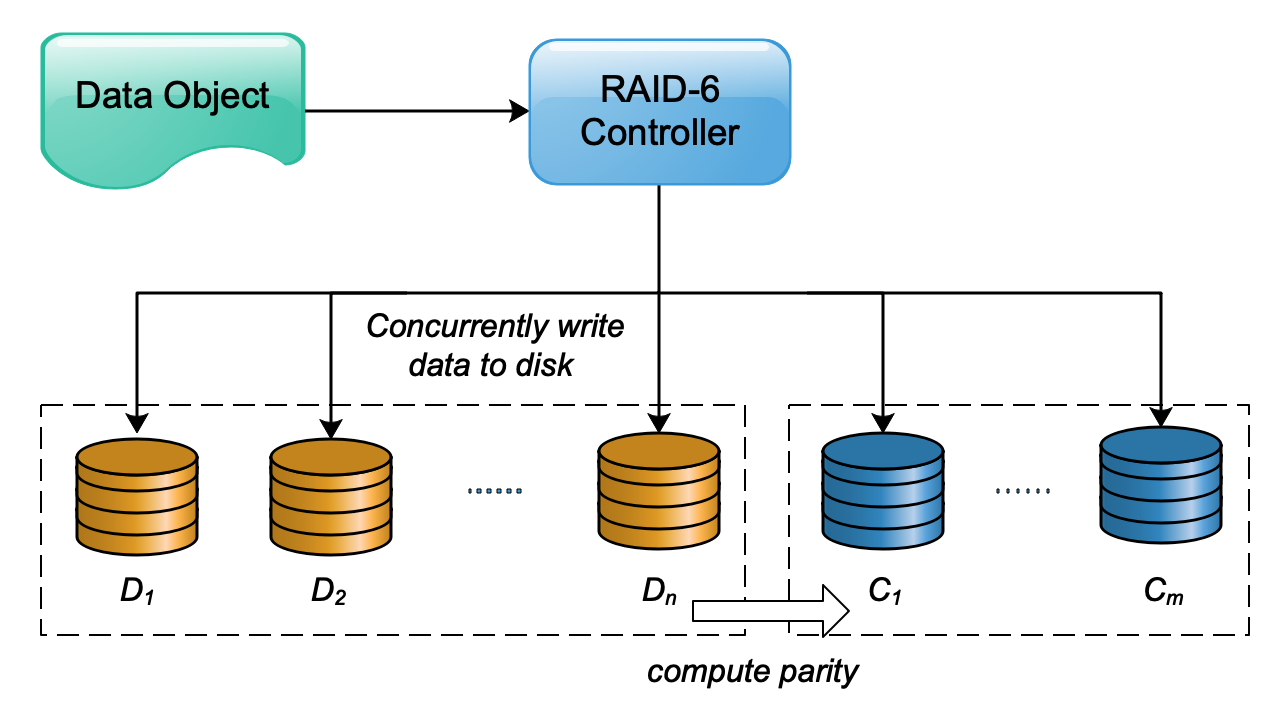
\includegraphics[width=0.5\textwidth]{fig/RAID-6.jpg}

	\caption{RAID-6 distributed storage system}

	\label{fig1}
\end{figure}


\section{Problem Specification}
\label{sec3}
The RAID-6 theory is based on the Galois Field mathematics and the Reed-Solomon codes. This section will provide relevant definations and principles in the implementation of a RAID-6 distributed storage system. The framework of a RAID-6 system is shown in Figure \ref{fig1}. First, let $D_1, D_2, ... , D_n$ denote $n$ \emph{storage disks} and $C_1, C_2, ... , C_m$ denote $m$ \emph{checksum disks}. Each of this disk holds the same storage capacity. The objective is to define the calculation of $C_i$ such that if any $m$ of $D_1, D_2, ... , D_n, C_1, C_2, ... , C_m$ corrupt. The contents of the corrupted devices can be rebuilt from the non-corrupted devices.

\subsection{Arithmetic over Galois Field}
Fields with $2^w$ elements under closed operations like addition and multiplication are called \emph{Galois Fields} (denoted as \textbf{GF($2^w$)}). The elements are integers from zero to $2^w-1$. For example, the field \textbf{GF(2)} can be represent as the set ${0,1}$. A small field would limit the number of disks possible while a large field would require extremely large tables. For RAID-6, we choose the commonly used field of \textbf{GF($2^8$)}, which allows for a maximum of 255 data disks. The operations in this finite field are illustrated as below:

\emph{Addition}: The addition field operator $(\oplus)$ is  performed by bitwise XOR. 

\emph{Subtraction}: The addition and subtraction $(\ominus)$ are the same operation. For example, $A \oplus B = A \ominus B$

\emph{Multiplication}: The multiplication $(\otimes)$ is performed by bitwise AND, and can be simplified using logarithms table. The details of setting up this table will be presented later.

\emph{Division}: Division is defined as multiplication with an inverse like $A/B = A \otimes B^{-1}$

Based on the definitions of the foundamental operations, the following basic rules should be obeyed in this field:

\begin{itemize}
	\item Addition is commutative: $A \oplus B = B \oplus A$
	\item Addition is associative:    $(A \oplus B) \oplus C = A \oplus (B \oplus C) $
	\item Multiplication is commutative: $A \otimes B = B \otimes A$
	\item Multiplication is associative: $(A \otimes B) \otimes C = A \otimes (B \otimes C)$
	\item  Distributive law: $(A \oplus B) \otimes C = A \otimes C  \oplus B \otimes C$
\end{itemize}

Here, we further explain how to perform multiplication and division in \textbf{GF($2^8$)}. The multiplication and division in this field is much more difficult and harder to implement. Multiplying two field elements is to multiply their corresponding polynominals. To simplify this calculation, we use two look up logarithm tables with length of each equals $2^w-1$. These tables are defined as \emph{gflog} and \emph{gfilog} and can be generated using Algorithm \ref{alg1}.

\begin{algorithm}
	\KwIn{$w=8$, $modulus=0b100011101$}
	\KwOut{two logarithm tables}
	max = $1<<w$ \\
	$b = 1$ \\
	\emph{gflog}, \emph{gfilog} = malloc(max)\\
	\For{$log = 0$ \KwTo max}
	{
		\emph{gflog}[$b$] = $log$\\
		\emph{gfillog}[$log$] = $b$\\
		$b$ = $b<<1$\\
		\If{$b$ \& max}{$b$ = $b$ \textsuperscript{$ \wedge $} $modulus$}
	}
	\caption{Setup logarithm tables}
	\label{alg1}
\end{algorithm}

\begin{itemize}
	\item \emph{gflog[]}: This table is defined for the indices 1 to 255, which maps the index to its logarithm in the Galois Field.
	\item \emph{gfilog[]}: This table is defined for the indices 0 to 254, which maps the index to its inverse logarithm in the Galois Field. 
\end{itemize}

Obviously, \emph{gflog[gfilog[i]] = i}, and \emph{gfilog[gflog[i]] =i}. With these two tables, we can easily multiply two non-zero elements of \textbf{GF($2^8$)} by adding their logs and then taking the inverse log as given by:

\begin{equation}
A \otimes B = gfilog[gflog[A] + gflog[B]]
\end{equation}

\begin{equation}
A \otimes B^{-1} = gfilog[gflog[A] - gflog[B]]
\end{equation}

When $w$ is small, these two tables can accelerate multiplication and division in the Galois Field.

\subsection{Reed-Solomen Coding}

By using Reed-Solomen Coding, we could use more parities to back up our data, not just 2. It could be very helpful when one wants to achieve better data security.

\subsubsection{Calculating Parities}

Suppose we have $N$ data disks and $M$ parity disks. To calculate the parity $P_i$, we define function $F_i$: 

\begin{equation}
P_i = F_i(d_1,d_2,...,d_n) = \sum_{j=1}^{n}d_j f_{i,j}
\end{equation}

If we treat data and parity as vectors, where $D = [d_1, d_2, ... , d_i]$ and $P = [p_1, p_2, ... ,p_i]$, we could get a simpler equation:

\begin{equation}
P=FD
\end{equation}

To calculate P, first, we need to generate the $M \times N$ Vandermonde matrix F where $f_{i,j} = j ^ {i-1}$

\begin{equation}
F =
\left[
\begin{matrix}
1      & 1      & \cdots & 1      \\
1      & 2      & \cdots & N      \\
\vdots & \vdots & \ddots & \vdots \\
1      & 2^{M-1}      & \cdots & N^{M-1}      \\
\end{matrix}
\right]
\end{equation}

In this way, we could easily get our parities $P$ by applying a matrix multiplication on Galois Field.

\subsubsection{Recovering Data}

To recover our data from disk faliure, we need to define matrix $A = \left[\begin{matrix}I \\F \\\end{matrix}\right]$ and $E= \left[\begin{matrix}D \\P \\\end{matrix}\right]$, where $I$ is a $N \times N$ identity matrix and matrix $F, D, P$ are defined before. So we get the equation:

\begin{equation}
AD=E
\end{equation}

When a disk or disks encount failure, we could delete the corresponding row in $A$ and $E$. For instance, we have one failed data disk $D_i$ and one failed parity disk $P_j$, then we need to delete $i_{th}$ row in $I$ and $j_{th}$ row in $F$ to get a new $A'$. Likewise, we also need to delete $i_{th}$ row in $D$ and $j_{th}$ rwow in $P$ to get a new $E'$. Then the equation becomes: 

\begin{equation}
A'D=E'
\end{equation}

What we want is actually D, so the problem becomes to solve the following equation:

\begin{equation}
D=A'^{-1}E'
\end{equation}

The way we use to calculate the inverse matrix $A'^{-1}$ is Gaussian Elimination, the only difference is we do it in Galois Field. Once we calculate our data D, then by using the method mentioned before: $P=FD$, we could update our parity P if it's necessary. 

\section{ Implementation}
\label{sec4}

\subsection{System Configuration}
The configuration of the RAID-6 based distributed storage system is shown below
\begin{itemize}
	\item Number of Disks: $N$ = 6
	\item Number of Data Disks: $D$ = 4
	\item Number of Parity Disks: $C$ = 2
	\item $D_1 \sim D_6$ denote 6 disks
	\item Chunk Size: 16 Bytes
\end{itemize}

Furthermore, one could change the configuration such as number of parity disks or chunk size to extend RAID6 system. On chunk size, when there are mainly large files to be stored, it is recommended to use a larger chunk size.

To fully distribute our data in all disks, we will shift our data chunk and parity chunk in one direction. Each stripe of data includes D(which is 4 in our configuration) raw data chunk: $d_{ij}$ where $i$ is chunk index and $j$ is stripe index, and C(which is 2) parity chunk: $p_{ij}$. And the order of data chunk and parity chunk will shift, which could average the IO pressure on all disks. If we do not shift the store location and assign some disks to only store parity data, they may be a big bottleneck if their IO speed is much slower than others.

\begin{table}[ht]
\centering
\begin{tabular}{c|cccccc}

 		&  $D_1$ 	& $D_2$ 	& $D_3$ 	& $D_4$ 	& $D_5$ 	& $D_6$ 	\\
 		\hline
 $S_1$ 	&  $d_{11}$ & $d_{21}$ 	& $d_{31}$ 	& $d_{41}$ 	& $p_{11}$ 	& $p_{21}$ 	\\
 $S_2$ 	&  $p_{22}$	& $d_{12}$ 	& $d_{22}$ 	& $d_{32}$ 	& $d_{42}$ 	& $p_{12}$ 	 \\
 $S_3$ 	&  $p_{13}$ & $p_{23}$	& $d_{13}$ 	& $d_{23}$ 	& $d_{33}$ 	& $d_{43}$ 	\\
 \vdots &   \vdots & \vdots & \vdots & \vdots & \vdots & \vdots  	
\end{tabular}
\caption{RAID6 data distribution}
\end{table}

\subsection{Basic Functions}

We first implemented some basic functions: data segmentation, writing, reading and recovering. With these functions, we could store a file in an abstract RAID6 system, and then read or recover it.

On data segmentation, every time we will read 4 chunks of data whose size should be $Chunk size \times Number Of Data Disks = 16 \times 4 = 64 Bytes$ from file. And then by applying Reed-Solomen algorithm, we could calculate the corresponding parity data chunks to compose a completed stripe. 

On writing, we need to shift it according to its stripe number. After successfully writing into RAID6, the total number of stripes and file information like file name and format should be recorded as well.

On reading and recovering, the most important part is to correctly indexing each chunk to decide its order in stripe. While reading, to make it faster, we could skip the parity data chunks if we do not need to check the completeness of file. While recovering, we could only compute the missing parts rather than computing all chunks.

\subsection{Other Functions}
In addition to basic functionalities, we also developed several advanced features in our RAID-6 distributed storage system. The advanced features we have implemented are summarized as fellows.

\subsubsection{Accommodate Real Files of Arbitrary Size} Previously, the data object we used for test is a synthetically generated string in .txt file. To make it available for practical storage, we have tried different data in other format. Zero padding method is included to ensure that files in different are equally distributed with respect to the chunk size of each disk. The padding  method added a series of bit 0 at the end of the files and can be clipped when rebuilding data from non-corroputed disks.

\subsubsection{Support User Defined Configurations } In the test phase, the RAID-6 system is specifically configured with 6 data disks and 2 checksum disks as the conventional example.  To make it more flexible, we separately take the configuration file as a Python class to let users define their preferred choice for practical implementation. The experiments of different configurations with different performance is discussed in Section \ref{sec5} . 

\section{Experiments}

\label{sec5}

In this experiment, we change the chunk size to \textbf{4 Bytes}, \textbf{8 Bytes}, ..., and \textbf{256 Bytes}. The test file we use is a jpg with size of 805 KB. We measure the reading, writing and recovering time in the configuration of 4 data disks and 2 parity disks. Following figures are the experiment result:


\begin{figure}[htbp]

	\centering

	\captionsetup{justification=centering}

	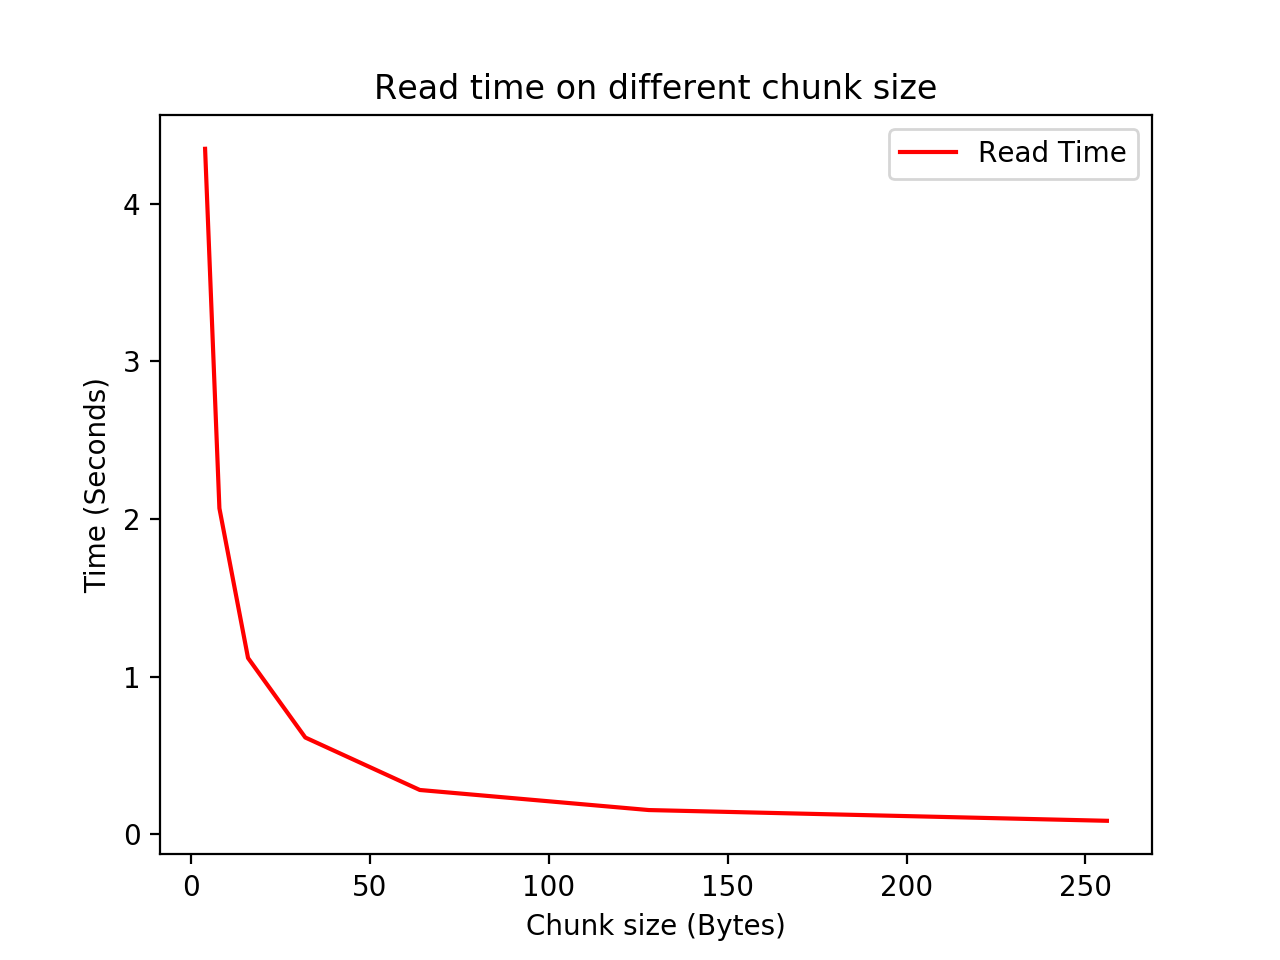
\includegraphics[width=0.4\textwidth]{fig/result_read.png}

	\caption{Read time on different chunk size, file size is 802 KB}

\end{figure}


\begin{figure}[htbp]

	\centering

	\captionsetup{justification=centering}

	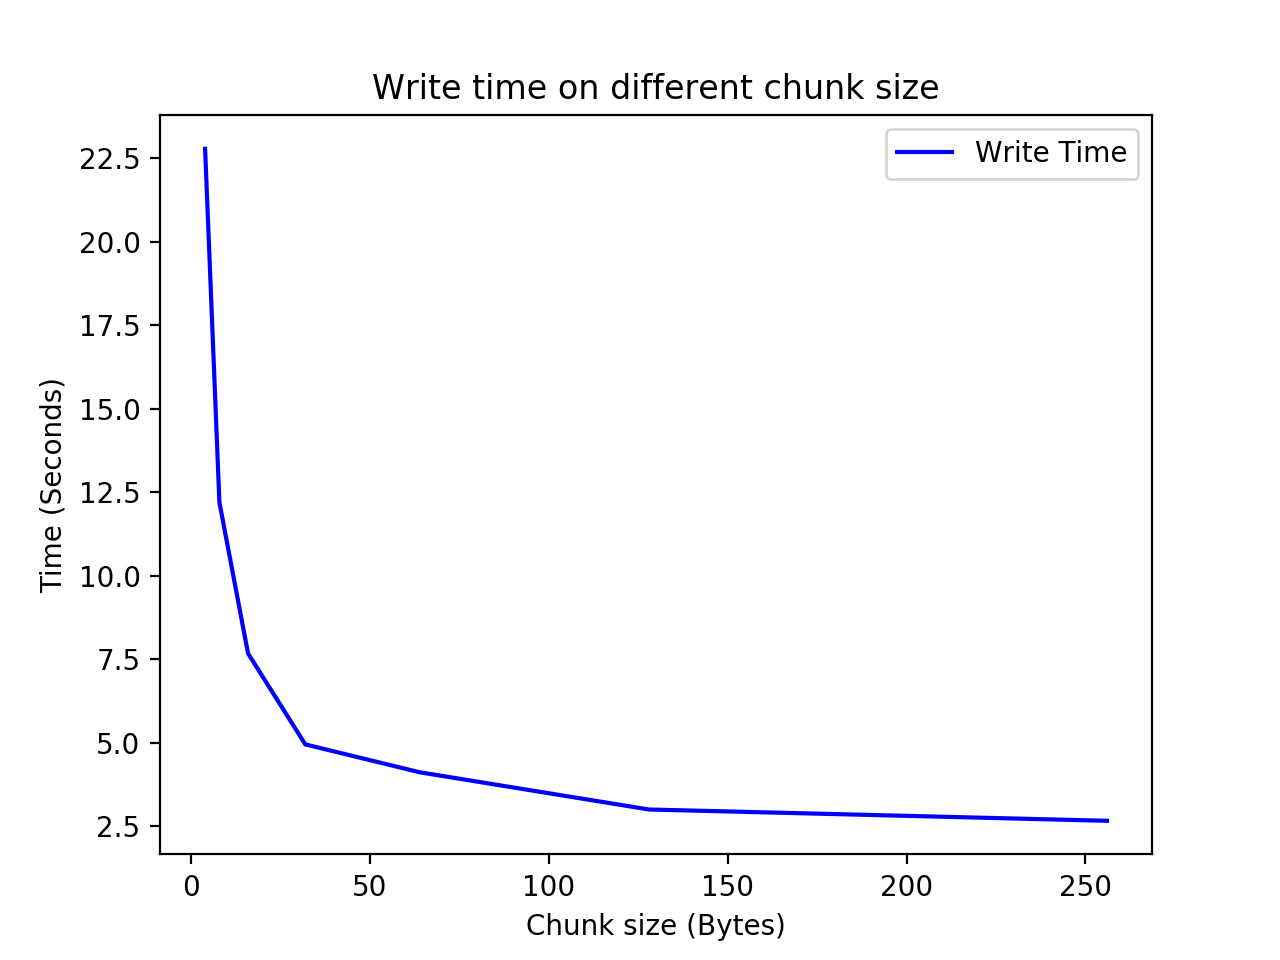
\includegraphics[width=0.4\textwidth]{fig/result_write.png}

	\caption{Write time on different chunk size, file size is 802 KB}

\end{figure}


\begin{figure}[]

	\centering

	\captionsetup{justification=centering}

	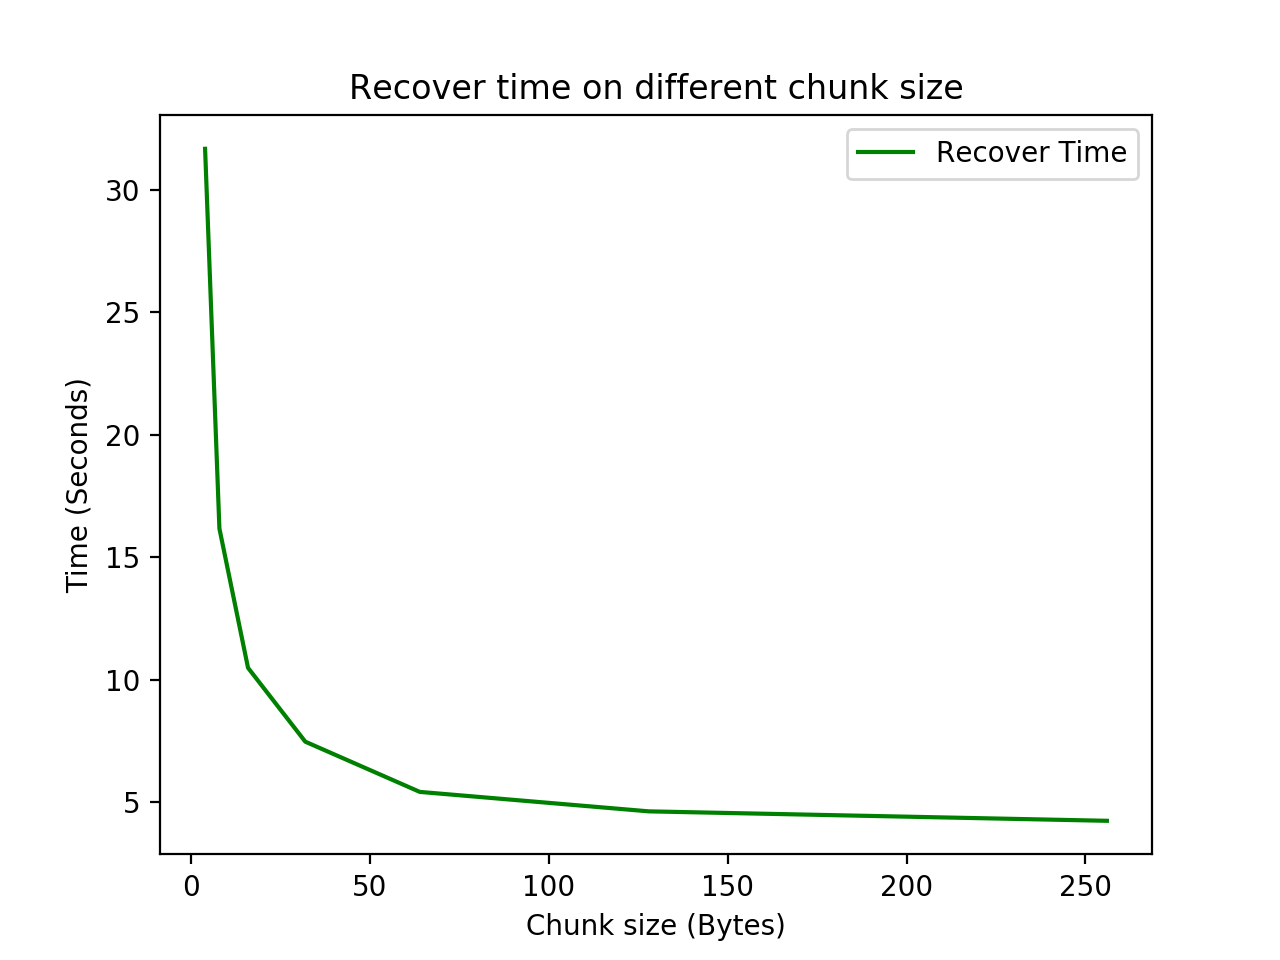
\includegraphics[width=0.4\textwidth]{fig/result_recover.png}

	\caption{Recover time on different chunk size, file size is 802 KB}

\end{figure}


In second experiment, we use the txt file with size of 512 Bytes, and measure the reading, writing and recovering time.


\begin{figure}[H]

	\centering

	\captionsetup{justification=centering}

	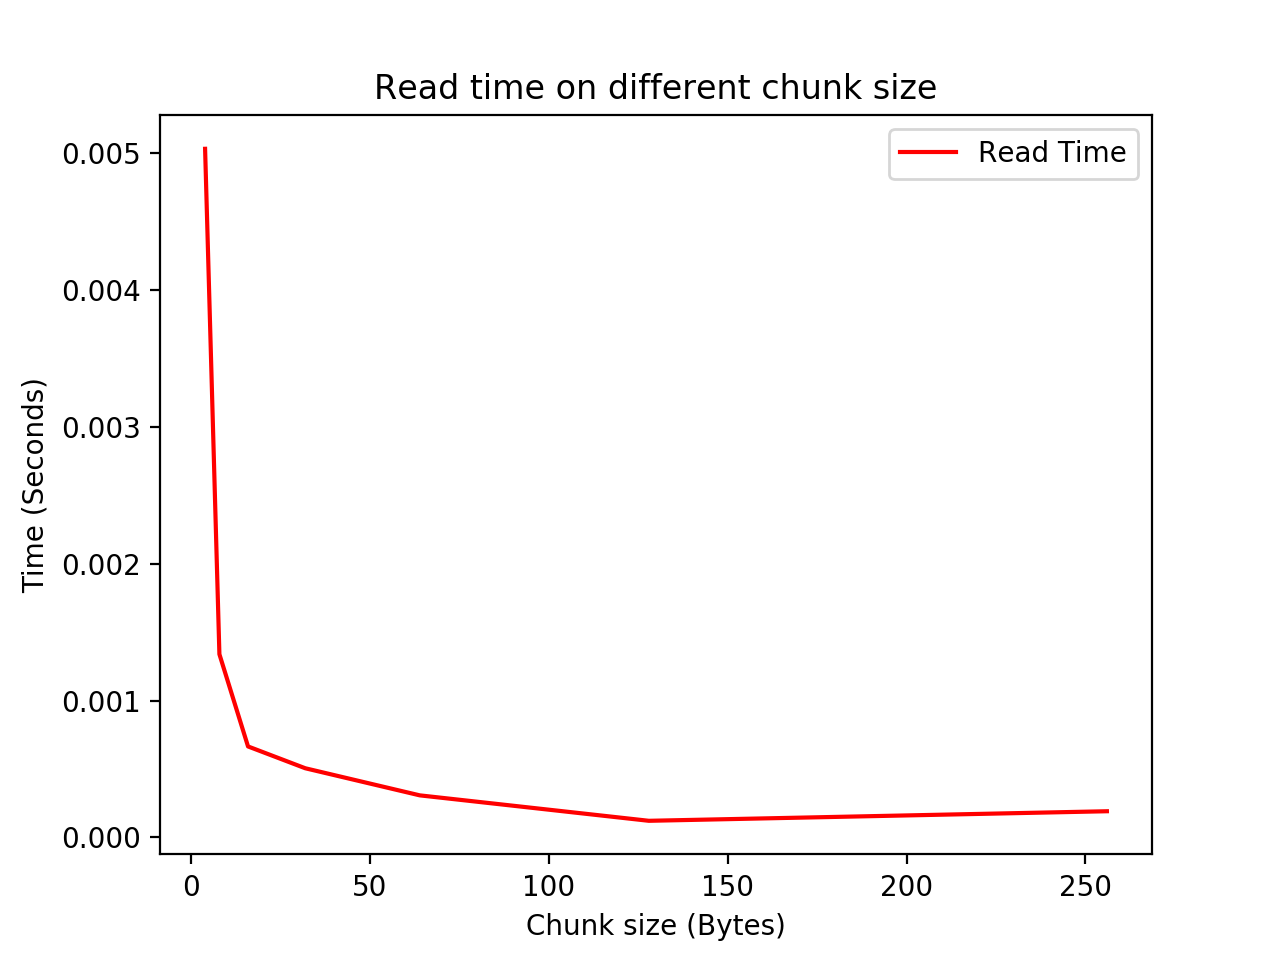
\includegraphics[width=0.4\textwidth]{fig/result_read_small.png}

	\caption{Read time on different chunk size, file size is 512 Bytes}

\end{figure}


\begin{figure}[H]

	\centering

	\captionsetup{justification=centering}

	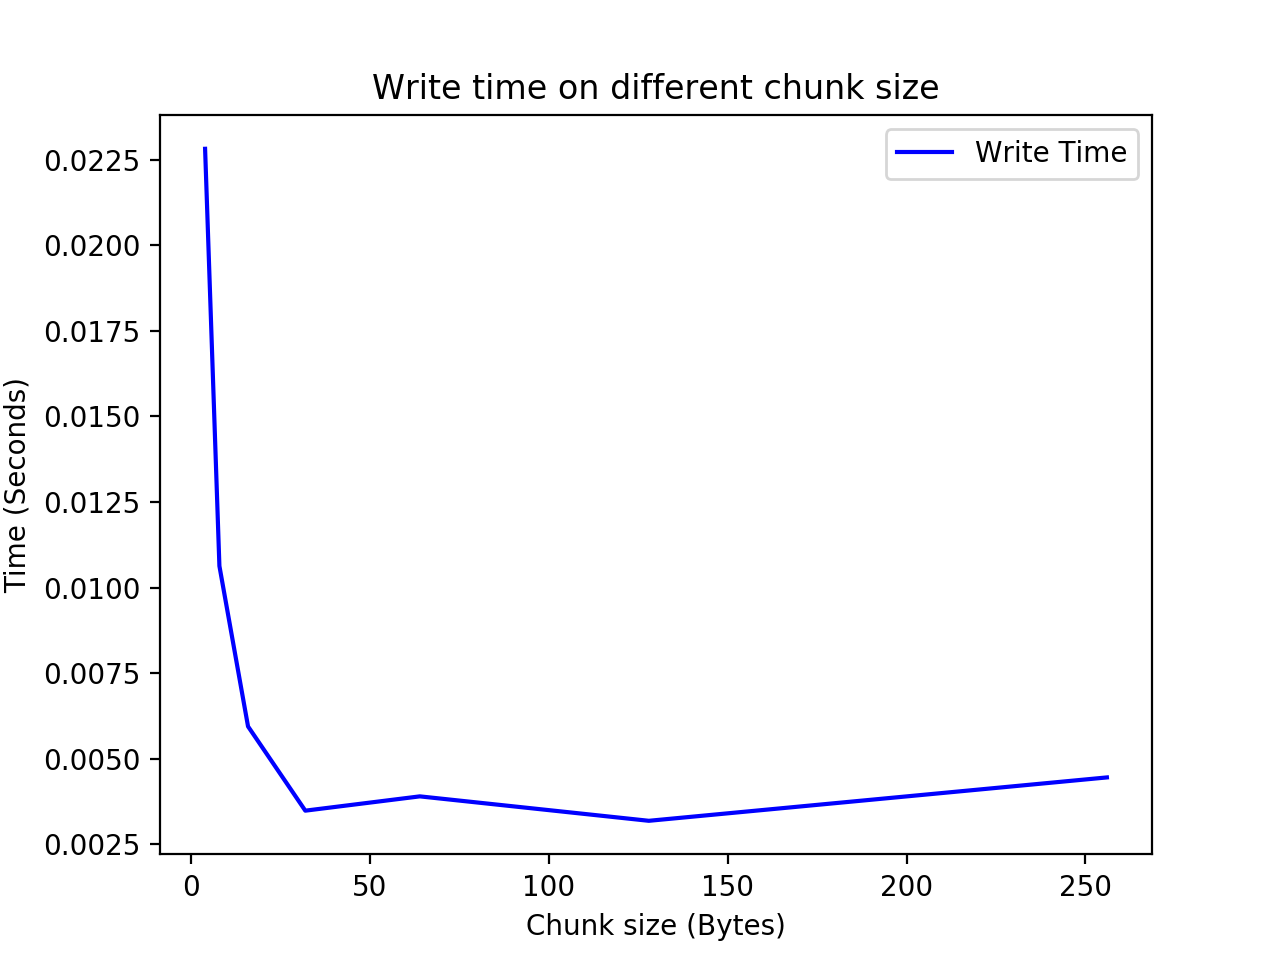
\includegraphics[width=0.4\textwidth]{fig/result_write_small.png}

	\caption{Write time on different chunk size, file size is 512 Bytes}

\end{figure}


\begin{figure}[H]

	\centering

	\captionsetup{justification=centering}

	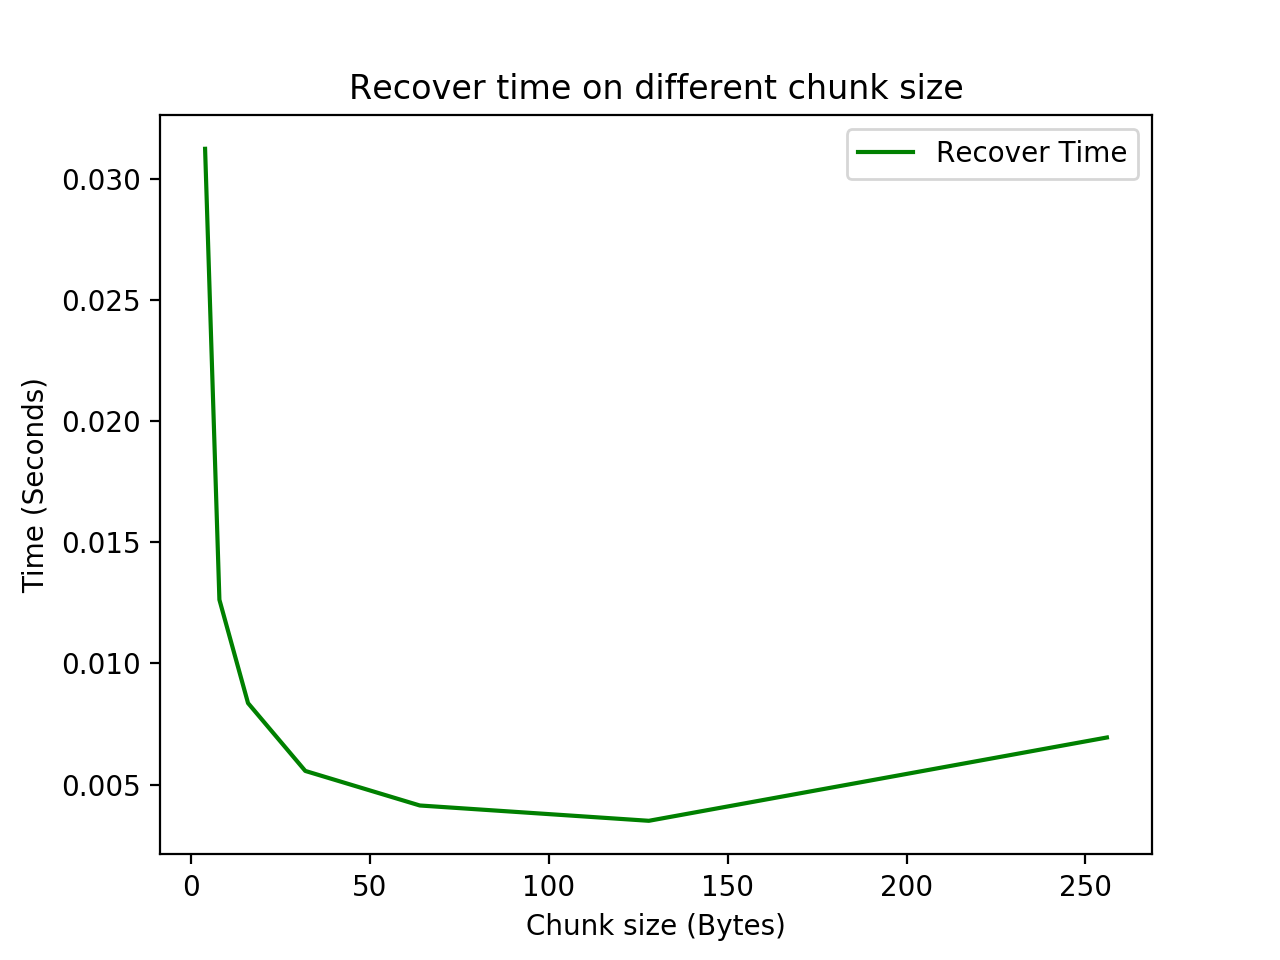
\includegraphics[width=0.4\textwidth]{fig/result_recover_small.png}

	\caption{Recover time on different chunk size, file size is 512 Bytes}

\end{figure}


From the results, we can see that with the chunk size becomes larger, the reading, writing and recovering time all decrease. This is because data is divided into larger pieces, which reduces the times of reading or writing the file(IO). However, in second experiment, when the chunk size is too large compared with the file size, the performance might be worse. So the chunk size should depend on how large you files mainly are. If you store many tiny files, smaller chunk size could save space because of less padding. On the contrary, larger chunk size should be choosed if there are many large files because of less IO time.


\section{Conclusion}
\label{sec6}
We have successfully developed a RAID-6 based distributed storage system in Python 3.7 under Linux environment. Instead of using existing finite field libraries, we create our own class for basic operations in Galois Field. Based on the mathematics of Reed-Solomen Coding, the RAID-6 system is able to support basic functionalities such as distributed data storage, failure detection and lost redundancy recovery. On top of the minimal implementation, we also develop several advanced features to make the system more flexiable and scalable. To make it available for impementation, we open source our codes at GitHub for further test and discussion.


% use section* for acknowledgment
\section*{Acknowledgment}
We would like to thank Prof. Anwitaman Datta for teaching the course CE7490 Advanced Topics in Distributed Systems and the abundant resources provided in his lecture.

\begin{thebibliography}{1}

\bibitem{IEEEhowto:kopka}
H.~Kopka and P.~W. Daly, \emph{A Guide to \LaTeX}, 3rd~ed.\hskip 1em plus
0.5em minus 0.4em\relax Harlow, England: Addison-Wesley, 1999.

\bibitem{RAID-6}
H. Peter Anvin, \emph{The mathematics of RAID-6}, 1st~ed, 20, Dec, 2011.

\bibitem{tutorial}
J. S. Plank, \emph{A Tutorial on Reed-Solomon Coding for Fault-Tolerance in RAID-like Systems},  University of Tennessee, July, 1996. \url{http://web.eecs.utk.edu/~jplank/plank/papers/CS-96-332.html}

\end{thebibliography}


\end{document}


